\setmainfont{Noto Serif}
\setsansfont{Noto Sans}
\setmonofont{Noto Sans Mono}
\setstretch{1.35}
\hyphenation{ма-те-ма-ти-ка вос-ста-нав-ли-вать}


\section{Применение теории возмущений}
1. Определите изменение порядка $\pi$-связи в молекуле этилена при введении в~его $\pi$-систему метильной группы.
\par
2С. Используя теорию возмущений определите вид нижней по энергии молекулярной орбитали в молекуле нафталина.
\par
3С. Определите изменение полной электронной энергии $\pi$-системы циклобутадиена, при изменении геометрии молекулы с плоской квадратной на~прямоугольную. Считать, что при таком искажении длины соответствующих связей изменились на 0,1 относительно неискаженной геометрии.
\par
4. Используя теорию возмущений определите распределение спиновой плотности в~анион-радикале п-терфенила.
\par
\begin{wrapfigure}{r}{36mm} %this figure will be at the right
    \centering
    \vspace{-7ex}
    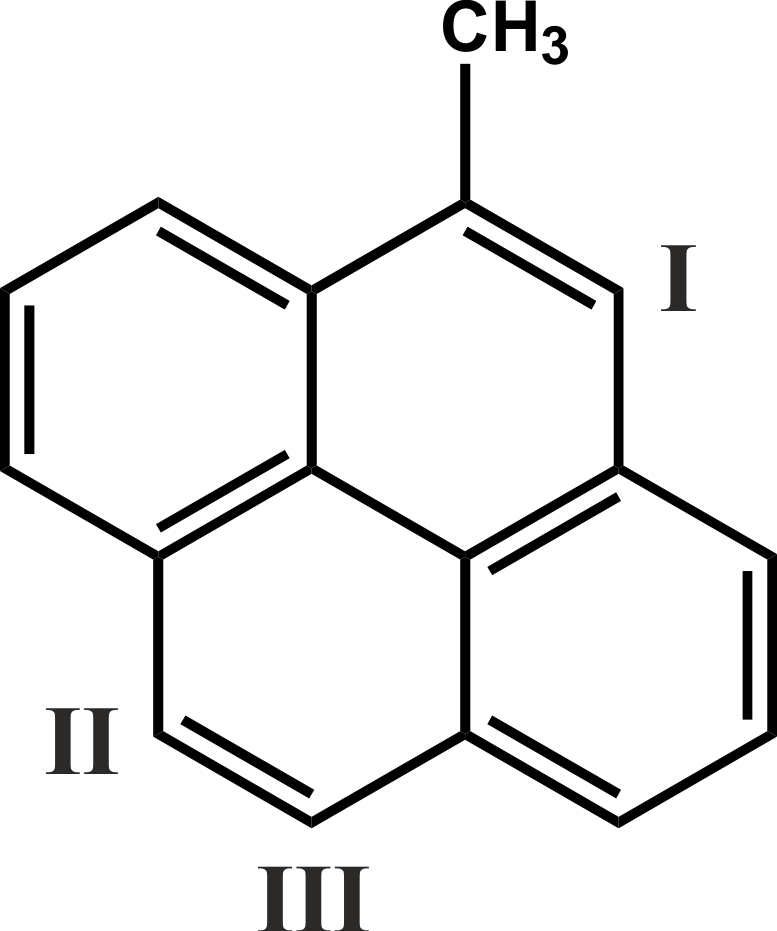
\includegraphics[width=20mm]{images/Fig_1_9_6.png}
    \vspace{-6ex}
\end{wrapfigure}
5К. В первом порядке теории возмущений определите преимущественное направление (центры I, II или III, см.~рисунок) электрофильного ароматического замещения в 4-метилпирене, $\xi$ = $-$0,1.
\par
6. Рассчитать распределение спиновой плотности в анион- и катион-радикале дурола (1,2,4,5-тетраметилбензола). Как изменится энергия и поляризация самого длинноволнового электрического дипольного перехода при переходе от бензола к дуролу?
\par
7. Используя теорию возмущений сравнить относительную устойчивость изомерных $\pi$-систем антрацена и фенантрена.
\par
8С. Определить направление преимущественного нуклеофильного ароматического замещения в 1-метил-2-трифторметил-циклобутадиене.
\par
\begin{wrapfigure}{r}{30mm} %this figure will be at the right
    \centering
    \vspace{-4ex}
    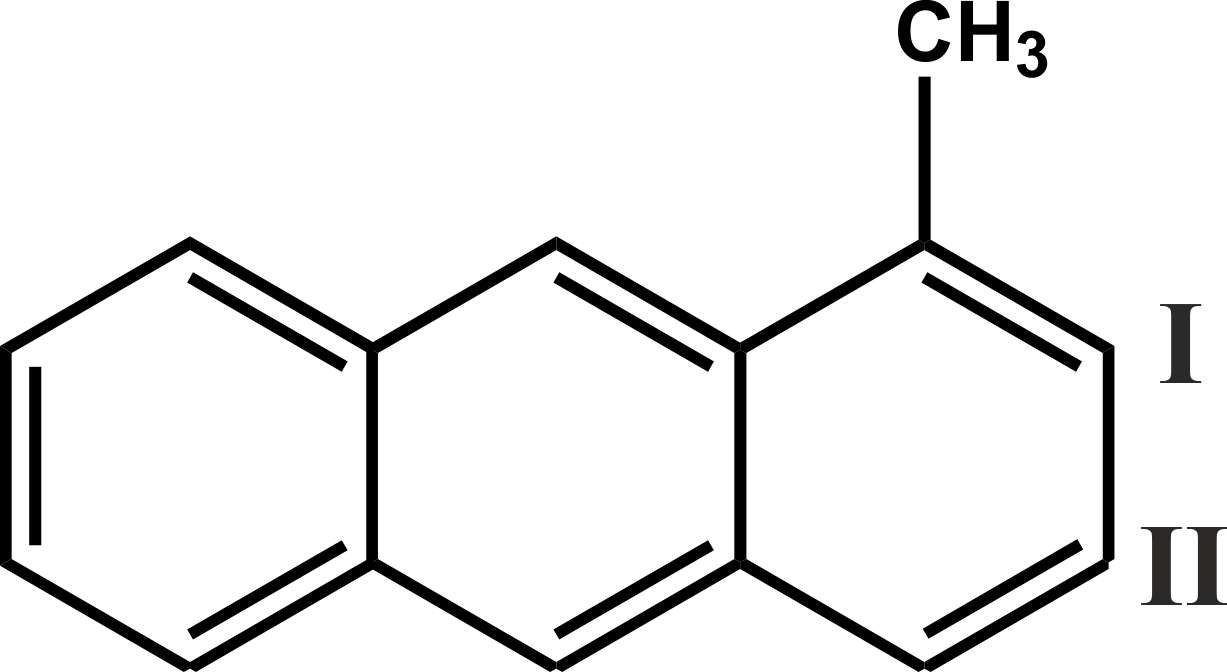
\includegraphics[width=27mm]{images/Fig_1_9_9.png}
    \vspace{-3ex}
\end{wrapfigure}
9К. В первом порядке теории возмущений определите преимущественное направление (центры I или II, см.~рисунок) нуклеофильного ароматического замещения (R$^-$) в~1-метилантрацене, $\xi$ = $-$0,1.
\par
10. В первом порядке теории возмущений определите преимущественное направление нуклеофильного и электрофильного ароматического замещения в~молекуле 4-трифторметилтолуола, $\xi_{\text{CH}_3}$ = $-$0,1, $\xi_{\text{CF}_3}$ = +0,3.
\par
\begin{wrapfigure}{r}{30mm} %this figure will be at the right
    \centering
    \vspace{-3ex}
    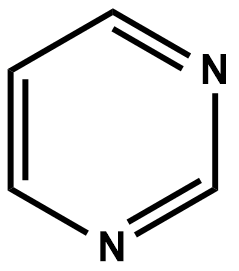
\includegraphics[width=10mm]{images/Fig_1_9_11.png}
    \vspace{-4ex}
\end{wrapfigure}
11Т. Опишите подходы к описанию электронного строения $\pi$-сопряженных соединений, имеющих в своей структуре один или несколько гетероатомов. В качестве примера рассчитайте изменение спиновой плотности в катион-радикале пиримидина, строение которого приведено на рисунке.
\par
12. Определите направление преимущественного электрофильного замещения для молекулы резорцина (1,3-дигидроксибензол). Считайте, что кулоновский интеграл для $2p_z$ атомной орбитали кислорода равен $\alpha_O=\alpha_C+1,2\beta$, резонансные интегралы для связи С–O равны $1,1\beta$.
\par
13. Определить преимущественный продукт одновременного радикального замещения водорода в бензоле двумя одинаковыми радикалами.
\par
14. Можно ли различить изомеры дважды дейтерированного бензола по энергии самой коротковолновой полосы поглощения $\pi$-системы?
\par
\begin{wrapfigure}{r}{30mm} %this figure will be at the right
    \centering
    \vspace{-4ex}
    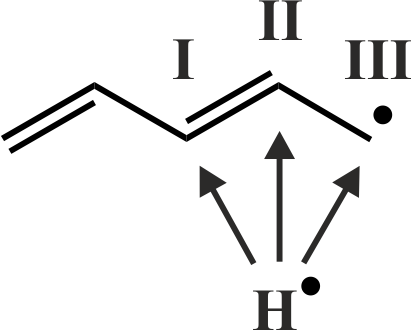
\includegraphics[width=18mm]{images/Fig_1_9_15.png}
    \vspace{-4ex}
\end{wrapfigure}
15К. Определите направление преимущественного присоединения (центры I, II или III, см. рисунок) атома водорода к $\pi$-системе пентадиенильного радикала.
\par